
%----------------------------------------------------------------------------
\chapter{Evaluation}
%----------------------------------------------------------------------------


\section{Measurement setup}

To measure the performance of the code generated by our framework we use the following setup.
We use 6 BeagleBone Black (BBB) \cite{BBB} as computation units. 
We connect them via network. 


\section{Measurement scenarios}

We generated models of size 45, 450, 4500, and 45000.

The models can partitioned to computation units in 3 different ways 
\begin{itemize}
	\item Standard -- The model is partitioned by equally distributing the model considering locality ie.\ elements that are connected have more probability of being allocated to the same unit
	\item Alternative -- The model is partitioned by equally distributing the model not considering locality
	\item Single -- All of the elements are allocated on the same computing unit
\end{itemize}

We measured on this 12 type of models 4 queries: \texttt{closeTrains}, \texttt{derailment}, \texttt{endOfSiding} and\texttt{trainLocations}. 
These were described in Section~\ref{sec:vql-examples}.
We measured the queries time of evaluation 10 times and took their average.

\pagebreak

\section{Results, and evaluation}

The results of the measurements can be seen on \autoref{fig:measurement-interpreted-code}.

\begin{figure}[h]
	\begin{center}
		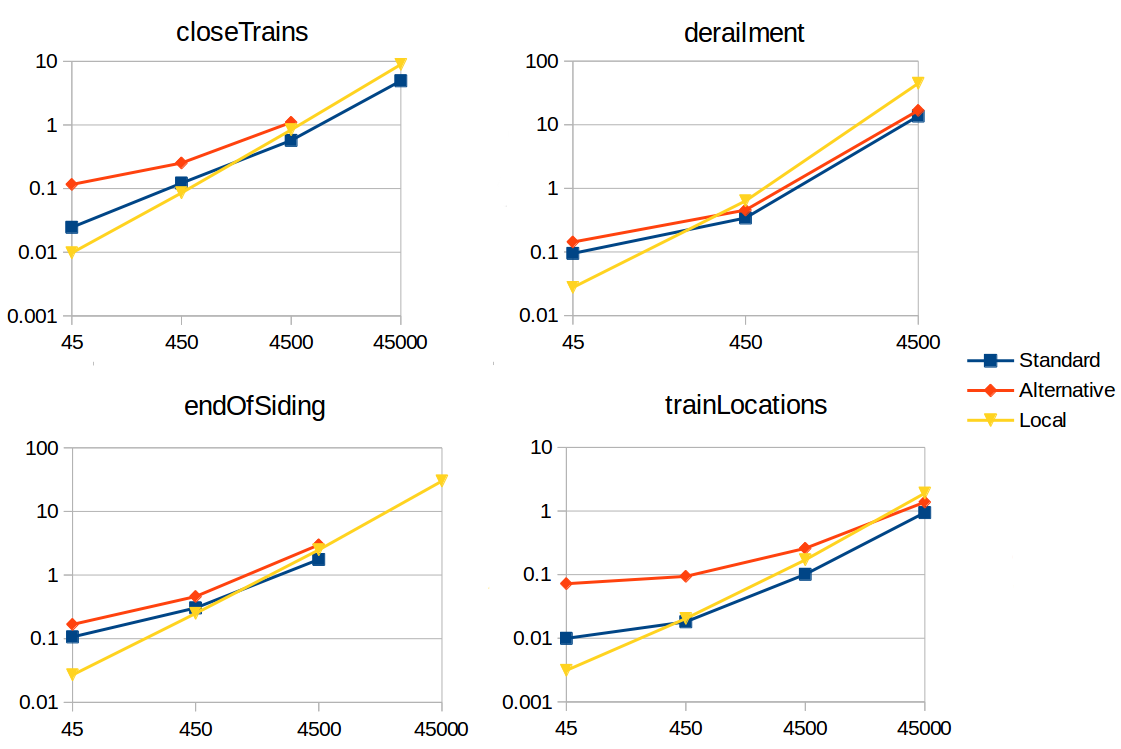
\includegraphics[width=\textwidth]{figures/measurement-interpreted-code.png}
		\caption{Example for edges between nodes}
		\label{fig:measurement-interpreted-code}
	\end{center}
\end{figure}

The fastest way most of the times were with standard model allocation: it indeed helped to run the queries faster. It was also faster than local evaluation, expect for \texttt{endOfSiding}, where only local model could be measured for the size of 45000, as at other models \texttt{endOfSiding} query was timeouted.

\texttt{trainLocations} and \texttt{closetrains} were faster queries: the reason is obviously the negated pattern call in other queries, which could not be implemented optimally for them.

